\documentclass{beamer}

% Code Segments
\usepackage{listings}
% Copyright 2017 Sergei Tikhomirov, MIT License
% https://github.com/s-tikhomirov/solidity-latex-highlighting/
\usepackage{listings, xcolor}

\newcommand\YAMLcolonstyle{\color{red}\mdseries}
\newcommand\YAMLkeystyle{\color{black}\bfseries}
\newcommand\YAMLvaluestyle{\color{blue}\mdseries}

\makeatletter

% here is a macro expanding to the name of the language
% (handy if you decide to change it further down the road)
\newcommand\language@yaml{yaml}

\expandafter\expandafter\expandafter\lstdefinelanguage
\expandafter{\language@yaml}
{
  keywords={true,false,null,y,n},
  keywordstyle=\color{darkgray}\bfseries,
  basicstyle=\YAMLkeystyle,                                 % assuming a key comes first
  sensitive=false,
  comment=[l]{\#},
  morecomment=[s]{/*}{*/},
  commentstyle=\color{purple}\ttfamily,
  stringstyle=\YAMLvaluestyle\ttfamily,
  moredelim=[l][\color{orange}]{\&},
  moredelim=[l][\color{magenta}]{*},
  moredelim=**[il][\YAMLcolonstyle{:}\YAMLvaluestyle]{:},   % switch to value style at :
  morestring=[b]',
  morestring=[b]",
  literate =    {---}{{\ProcessThreeDashes}}3
                {>}{{\textcolor{red}\textgreater}}1     
                {|}{{\textcolor{red}\textbar}}1 
                {\ -\ }{{\mdseries\ -\ }}3,
}

% switch to key style at EOL
\lst@AddToHook{EveryLine}{\ifx\lst@language\language@yaml\YAMLkeystyle\fi}
\makeatother

\newcommand\ProcessThreeDashes{\llap{\color{cyan}\mdseries-{-}-}}

\usepackage{xcolor}
\definecolor{verylightgray}{gray}{0.95} 
% Images
\usepackage{graphicx}

% Sequence Diagram
\usepackage{geometry}
\usepackage{pgf-umlsd}
\usetikzlibrary{calc}

\usecolortheme{beaver}

\AtBeginSection
{
  \begin{frame}
    \frametitle{Table of Contents}
    \tableofcontents[currentsection]
  \end{frame}
}

\setbeamertemplate{itemize items}{\textbullet}
\setbeamertemplate{footline}[text line]{%
  \parbox{\linewidth}{\vspace*{-8pt}
    \insertshorttitle\hfill\insertshortauthor\hfill\insertframenumber
  }
}
\setbeamertemplate{navigation symbols}{}

\begin{document}

\title{Alternative scalable HIDS with investigation capability}
\subtitle{FIDS - Forensic-based Intrusion Detection System}
\author{Julian Stampfli}

\frame{\titlepage}


\begin{frame}
  \frametitle{Table of Contents}
  \tableofcontents
\end{frame}

%%%%%%%%%%%%%%%%%%%%%%%%%%%%%%%%%%%%%%%%%%%%%%%%%%%%%%%%%%%%%%%%%%%%%%%%%%%%%%%%
\section{Introduction}
%%%%%%%%%%%%%%%%%%%%%%%%%%%%%%%%%%%%%%%%%%%%%%%%%%%%%%%%%%%%%%%%%%%%%%%%%%%%%%%%

\begin{frame}[fragile]
  \frametitle{Intrusions}
  \begin{itemize}
    \item What?
    \begin{itemize}
      \item Malware
      \item Hacker
      \item Insider Threats
    \end{itemize}
    \pause
    \item Protection 
    \begin{itemize}
      \item Firewals
      \item Least privilege
      \item ...
    \end{itemize}

    \item Secure\pause ?
    \begin{itemize}
      \item Open Ports
      \item Weak Passwords
      \item Insecure Applications
      \item ...
    \end{itemize}
  \end{itemize}
\end{frame}

\begin{frame}[fragile]
  \frametitle{Intrusion Detection}
  \begin{columns}
    \begin{column}{0.5\textwidth}
      Network-Based
      \begin{itemize}
        \item Central scanning
        \item Uses
        \begin{itemize}
          \item Traffic Load
          \item Connections
          \item Inspection
        \end{itemize}
        \item Mainly pattern driven
      \end{itemize}
    \end{column}
    \begin{column}{0.5\textwidth}
      Host-Based
      \begin{itemize}
        \item Distributed Scanning 
        \item Uses
        \begin{itemize}
          \item Processes
          \item Files
          \item Network Configuration
        \end{itemize}
        \item Change driven
      \end{itemize}
    \end{column}
  \end{columns}
\end{frame}

\begin{frame}[fragile]
  \frametitle{HIDS - FIM}
  \begin{columns}
    \begin{column}{1\textwidth}
      Finding Changes
      \begin{itemize}
        \item Hashing to the rescue! \pause or not?
      \end{itemize}
    \end{column}
  \end{columns}
\end{frame}

\begin{frame}[fragile]
  \frametitle{Hashing}
  \begin{columns}
    \begin{column}{1\textwidth}
      \begin{itemize}
        \item Highly reliable
        \item Used for cryptographic use cases
        \item Fast? \pause - Yes but not really.
        \item FIM using Hashing?
        \begin{itemize}
          \item Tripwire - 1992 - Gone comercial
          \item Aide / Samhain - Current Opensource alternatives
        \end{itemize}
      \end{itemize}
    \end{column}
  \end{columns}
\end{frame}


\begin{frame}[fragile]
  \frametitle{HIDS - FIM}
  \begin{columns}
    \begin{column}{1\textwidth}
      Finding Changes
      \begin{itemize}
        \item Hashing
        \item Filesystem attributes to the rescue
      \end{itemize}
    \end{column}
  \end{columns}
\end{frame}

\begin{frame}[fragile]
  \frametitle{TSK}
  \begin{columns}
    \begin{column}{1\textwidth}
      The Sleuth Kit.
      \begin{itemize}
        \item Opensource
        \item Disk analyzis utility
        \item Used in forensics
      \end{itemize}
    \end{column}
  \end{columns}
\end{frame}

%%%%%%%%%%%%%%%%%%%%%%%%%%%%%%%%%%%%%%%%%%%%%%%%%%%%%%%%%%%%%%%%%%%%%%%%%%%%%%%%
\section{Forensic-based Intrusion Detection System (FIDS)}
%%%%%%%%%%%%%%%%%%%%%%%%%%%%%%%%%%%%%%%%%%%%%%%%%%%%%%%%%%%%%%%%%%%%%%%%%%%%%%%%


\begin{frame}[fragile]
  \frametitle{FIDS - Architecture}
  \begin{columns}
    \begin{column}{1\textwidth}
      \begin{figure}[ht]
        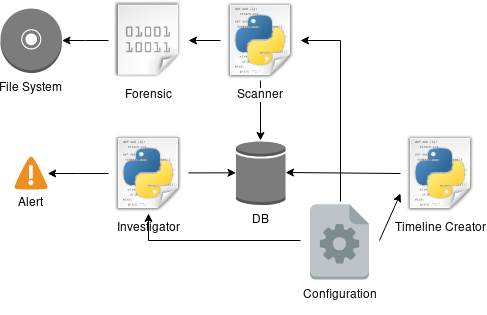
\includegraphics[width=8cm]{../img/Overview_FIDS.png}
        \centering
        \caption{System Architecture}
        \label{fig:systemArchitecture}
      \end{figure}
    \end{column}
  \end{columns}
\end{frame}

\begin{frame}[fragile]
  \frametitle{Search Functionality}
  \begin{columns}
    \begin{column}{1\textwidth}
      \begin{lstlisting}[language=python, numbers=left]
self.stack = []
for path in self.paths:
  open_dir_rec(get_entry(path))

def open_dir_rec(curDir):
  ...
  for entry in curDir:
    if entry.isDir and inode not in self.stack:
      self.open_directory_rec(entry)
    else:
      ...
      \end{lstlisting}
    \end{column}
  \end{columns}
\end{frame}

\begin{frame}[fragile]
  \frametitle{Run comparison query}
  \begin{columns}
    \begin{column}{1\textwidth}
      \begin{lstlisting}[language=sql, numbers=left]
  SELECT first.*, second.* 
  FROM FIDS_FILE first 
    LEFT JOIN FIDS_FILE second 
      on 
        (first.meta_addr=second.meta_addr 
          or first.path=second.path 
            and first.name_name=second.name_name) 
  WHERE first.run_id = ? 
    and second.run_id = ? 
    or first.run_id is null;
      \end{lstlisting}
    \end{column}
  \end{columns}
\end{frame}

\begin{frame}[fragile]
  \frametitle{Investigator Configuration}
  \begin{columns}
    \begin{column}{1\textwidth}
      \begin{lstlisting}[language=yaml, numbers=left]
  investigator:
    same_config: True
    rules: 
      - name: all_files
        rules: 
        equal: [meta_size]
        greater: 
    investigation:
      - paths:
          - '/'
        rules:
          - all_files
      \end{lstlisting}
    \end{column}
  \end{columns}
\end{frame}

\begin{frame}[fragile]
  \frametitle{Timeline Architecture}
  \begin{columns}
    \begin{column}{1\textwidth}
      MD5|name|inode|mode|UID|GID|size|atime|mtime|ctime|crtime
      \begin{lstlisting}[language=python, numbers=left]
print(
      '0|'
      f'{f.path}{f.name_name}|'
      f'{f.meta_addr}|'
      f'{mode}|'
      f'{f.meta_uid}|'
      f'{f.meta_gid}|'
      f'{f.meta_size}|'
      f'{f.meta_access_time}|'
      f'{f.meta_modification_time}|'
      f'{f.meta_changed_time}|'
      f'{f.meta_creation_time}')
      \end{lstlisting}
    \end{column}
  \end{columns}
\end{frame}

%%%%%%%%%%%%%%%%%%%%%%%%%%%%%%%%%%%%%%%%%%%%%%%%%%%%%%%%%%%%%%%%%%%%%%%%%%%%%%%%
\section{Summary/Conclusion}
%%%%%%%%%%%%%%%%%%%%%%%%%%%%%%%%%%%%%%%%%%%%%%%%%%%%%%%%%%%%%%%%%%%%%%%%%%%%%%%%

\begin{frame}[fragile]
  \frametitle{Challenges}
    \begin{itemize}
      \item Pytsk and TSK API Documentation
      \item Scan
      \item Thesis Document
    \end{itemize}
\end{frame}

\begin{frame}[fragile]
  \frametitle{Conclusion}
  \begin{columns}
    \begin{column}{1\textwidth}
      Summary
      \begin{itemize}
          \item Fast Scans
          \item Intrusion Detection Possible
          \item Support for Forensic Investigation
      \end{itemize}
      \pause
      Conclusion
      \begin{itemize}
        \item Risk-Based Approach
        \item Speed vs Reliability
      \end{itemize}
    \end{column}
  \end{columns}
\end{frame}

\begin{frame}[fragile]
  \frametitle{Further Research}
    \begin{itemize}
      \item Extension beyond Files
      \item Extensive Testing in a Live Environment
      \item Extend support for FS specific attributes
      \item Use more sophisticated storage solution
    \end{itemize}
\end{frame}


\begin{frame}
  \frametitle{Thank you for listening / Demo}
  Code: \url{https://github.com/Tartori/fids}
\end{frame}

\end{document}
